\documentclass{article}

\usepackage{../.template/summary}

\subject{Security by Design}
\semester{Winter 2024}
\author{Leopold Lemmermann}

\usepackage{pdfpages}

\begin{document}\createtitle

\includepdf[pages={14-16,18-19,21-29,31-32,35,37-38,40-41}, nup=3x7]{slides.pdf}
\part{Kryptographie}
\section{Grundlagen}
\subsection{Angriffsarten (schwer zu leicht)}
\begin{enumerate}
  \item \textbf{Ciphertext Only}: Angreifer kennt nur den Schlüsseltext
  \item \textbf{Known Plaintext}: Angreifer kennt Schlüsseltext und Klartext
  \item \textbf{Chosen Plaintext}: Angreifer kann Klartext wählen und erhält den Schlüsseltext (nicht-adaptiv: alle Klartexte müssen vorher gewählt werden)
\end{enumerate}

\subsection{Brechen (stark zu schwach)}
\begin{enumerate}
  \item \textbf{Vollständig}: Schlüssel gefunden
  \item \textbf{Universell}: Äquivalenter Schlüssel gefunden
  \item \textbf{Selektiv}: Bestimmte Nachricht entschlüsselt
  \item \textbf{Existenziell}: Irgendeine Nachricht entschlüsselt
\end{enumerate}

\subsection{Ziele}
\begin{itemize}
  \item \textbf{Verschlüsselung}: Vertraulichkeit
  \item \textbf{Signatur}: Integrität, Authentizität
\end{itemize}

\subsection{Klassische Chiffren}
\begin{itemize}
  \item \textbf{Transposition}: Veränderung der Reihenfolge
  \item \textbf{Subsitution}: Ersetzen von Zeichen
  \item \textbf{Produkt}: Kombination von Transposition und Substitution
\end{itemize}

\begin{enumerate}
  \item \textbf{Skytala}: Transposition mit Zylinderdurchmesser als Schlüssel
  \item \textbf{Polybios}: Substitution mit 5x5-Quadrat
  \item \textbf{Caesar}: Substitution mit Verschiebung
  \item \textbf{Vigenére}: Substitution mit Schlüsselwort
  \item \textbf{Beaufort}: involutorischer Vigenére (gleiche Verschlüsselung und Entschlüsselung)
  \item \textbf{Vernam} (one-time pad): Substitution mit zufälligem Schlüssel mit Klartextlänge
\end{enumerate}



\includepdf[pages={44-108}, nup=4x9]{slides.pdf}
\section{Symmetrische Systeme}
\begin{itemize}
  \item \textbf{Vollständigkeit}: Jedes Output-Bit hängt von jedem Input-Bit ab
  \item \textbf{Avalanche}: Jede Änderung im Input führt zu vielen Änderungen im Output
  \item \textbf{Nichtlinearität}: Output ist nicht linear abhängig vom Input
  \item \textbf{Korrelationsimmunität}: Keine Korrelation zwischen Input und Output
  \item \textit{sekundär}: Implementierbarkeit, Längentreue, Schnelligkeit
\end{itemize}

\subsection{Feistel-Prinzip}
\begin{figure}
  \centering
  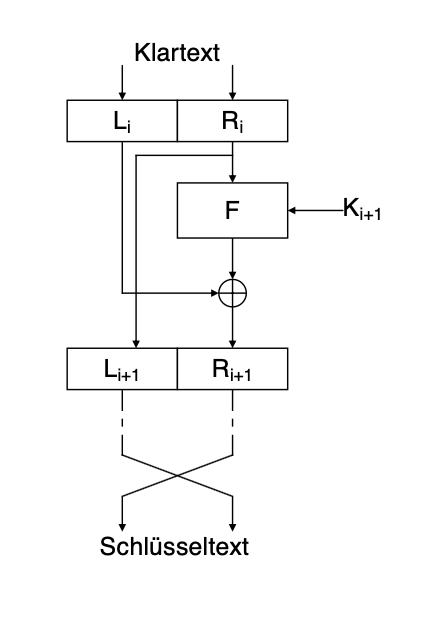
\includegraphics[width=.2\textwidth]{res/feistel.png}
  \caption{Feistel-Netzwerk}
  \label{fig:feistel}
\end{figure}

\subsection{DES (Data Encryption Standard)}
\begin{itemize}
  \item[+] vollständig
  \item[+] kein analytischer Zusammenhang zwischen Input und Output
  \item[+] invariant ggü. Komplementbildung
  \item[-] Designkriterien nicht öffentlich (inzwischen bekannt)
  \item[-] ineffiziente Implementierung wg. Permutationen
  \item[-] Schlüssellänge zu kurz (56 Bit)
  \item \textbf{möglicher Angriff}: Known-Plaintext-Angriff mit $2^{57}$ Aufwand
\end{itemize}

\subsection{IDEA (International Data Encryption Algorithm)}
\begin{itemize}
  \item \textbf{Schlüssellänge}: 128-Bit-Blockchiffre, entwickelt als sicherer Ersatz für DES.
  \item \textbf{Struktur}: Verwendet eine Kombination aus XOR-, Addition- und Multiplikationsoperationen für hohe Sicherheit.
  \item \textbf{Sicherheitsvorteile}: Resistenz gegen lineare und differentielle Kryptoanalyse.
  \item \textbf{Verwendung}: Besonders populär in Europa und wurde in PGP (Pretty Good Privacy) integriert.
\end{itemize}

\subsection{AES (Advanced Encryption Standard)}
\begin{itemize}
  \item \textbf{Schlüssellänge}: Unterstützt 128, 192 und 256 Bit, damit für verschiedene Sicherheitsniveaus geeignet.
  \item \textbf{Struktur}: Verwendet 10, 12 oder 14 Runden von Byte-Substitution, Zeilenverschiebung, Spaltenmischung und Rundenschlüssel-Addition.
  \item \textbf{Sicherheitsniveau}: Sicher gegen Brute-Force- und bekannte Kryptoangriffe, empfohlen von NIST als sicherer Standard.
  \item \textbf{Verwendung}: Weltweiter Standard für Verschlüsselung in Regierung, Industrie und dem Finanzsektor.
\end{itemize}

\subsection{Betriebsarten}
\begin{figure}
  \centering
  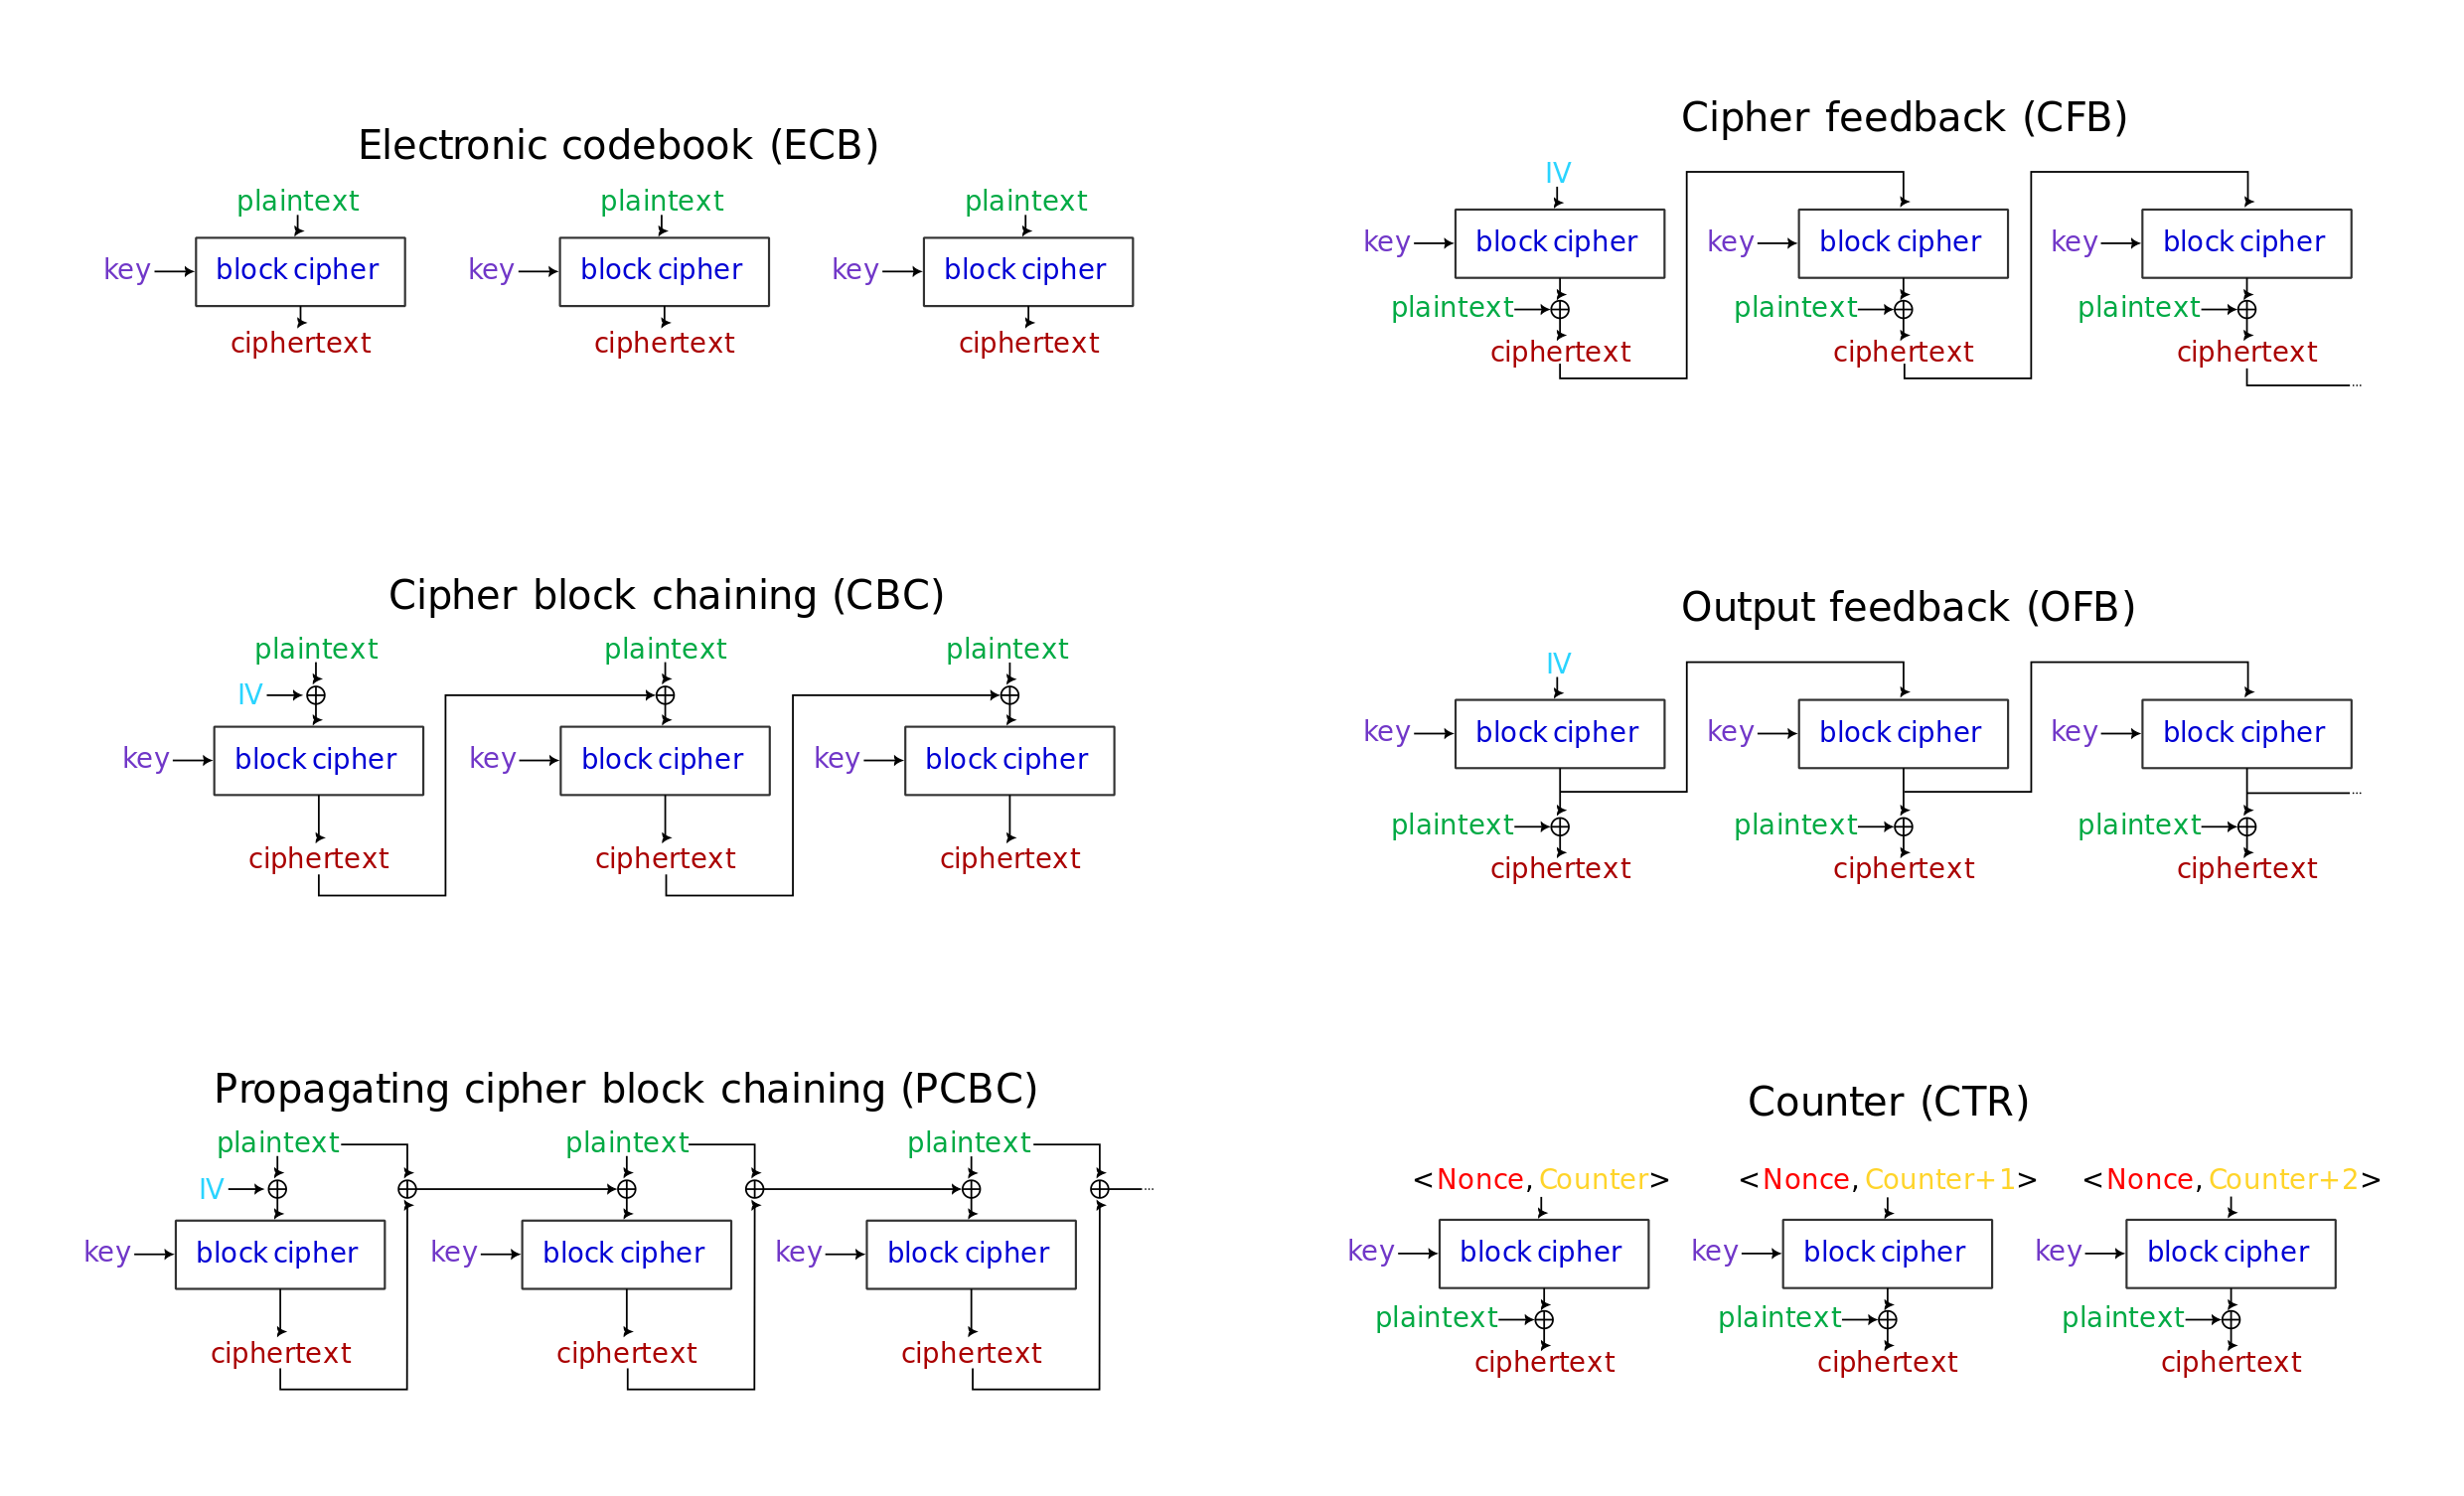
\includegraphics[width=.6\textwidth]{res/betriebsarten.png}
  \caption{Betriebsarten von Blockchiffren}
  \label{fig:betriebsarten}
\end{figure}
\begin{enumerate}
  \item \textbf{ECB (Electronic Codebook Mode)}: Klartext wird in Blöcke geteilt und einzeln verschlüsselt
  \item \textbf{CBC (Cipher Block Chaining Mode)}: Klartext wird in Blöcke geteilt und XOR-verknüpft
  \item \textbf{CTR (Counter Mode)}: Klartext wird in Blöcke geteilt und mit Zähler verschlüsselt
  \item \textbf{OFB (Output Feedback Mode)}: Klartext wird in Blöcke geteilt und mit Zähler verschlüsselt
  \item \textbf{CFB (Cipher Feedback Mode)}: Klartext wird in Blöcke geteilt und mit Zähler verschlüsselt
\end{enumerate}



\includepdf[pages={44, 109-142}, nup=4x9]{slides.pdf}
\section{Asymmetrische Systeme}
\begin{itemize}
  \item \textbf{Erweiterter Euklidischer Algorithmus}: ggT berechnen und erweiterter Algorithmus für Inverse
    \[ c_k=\lfloor\frac{r_{k-2}}{r_{k-1}}\rfloor \quad r_k = r_{k-2} \pmod{r_{k-1}} \quad s_k=s_{k-2}-c_ks_{k-1} \quad t_k=t_{k-2}-c_kt_{k-1} \]
  \item \textbf{Euler-Phi-Funktion}: $\varphi(n)$ gibt die Anzahl der zu $n$ teilerfremden (engl. coprime) Zahlen kleiner als $n$ an.
    \[ \varphi(p \cdot q) = (p-1) \cdot (q-1) \quad \text{Primzahlen: }\varphi(p) = p-1 \]
  \item \textbf{Primitive Wurzel}: Teilerfremdes $a$ ist primitive Wurzel modulo $n$, da $a^d \pmod{n}$ alle Reste erzeugt. Auch übertragen als:
    \[ a^d \not\equiv 1 \pmod{n} \text{ für } 1 \leq d < \varphi(n) \]
  \item \textbf{Diskreter Logarithmus}: $c$ ist diskreter Logarithmus von $a$ zur Basis $b$ modulo $n$:
    \[ b^c \equiv a \pmod{n} \to c = \log_b a \pmod{n} \]
  \item \textbf{Faktorisierungsannahme}: Primzahlen $p$ und $q$ sind schwer aus $n=p \cdot q$ zu berechnen.
  \item \textbf{(diskrete) Elliptische Kurve}: Eine elliptische Kurve über $\mathbb{Z}_p$ ist definiert durch
    \[ y^2 \equiv x^3 + ax + b \pmod{p} \text{ und } -4a^3 - 27b^2 \not\equiv 0 \pmod{p} \]
\end{itemize}

\subsection{Diffie-Hellman Key-Exchange}
\begin{figure}
  \centering
  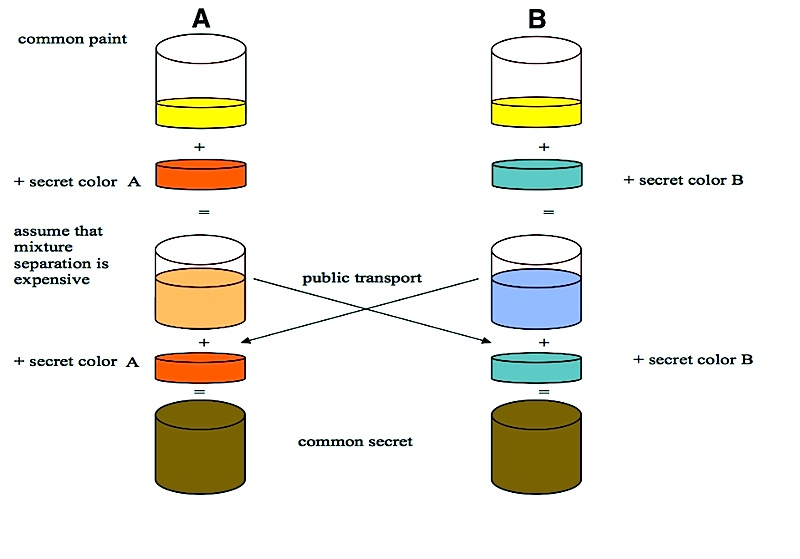
\includegraphics[width=.6\textwidth]{res/diffiehellman.jpg}
  \caption{Diffie-Hellman key exchange}
  \label{fig:diffiehellman}
\end{figure}

\subsection{ElGamal Verschlüsselung}
\textit{Basiert auf diskretem Logarithmus und Diffie-Hellman Key-Exchange. Einsatz zB. in GnuPG, PGP.}
\begin{itemize}
  \item \textbf{Parameter}
    \[
      \underbrace{\overbrace{x}^\text{zufällig}\in\mathbb{Z}^*_{p-1}}_\text{geheim}\quad
      \underbrace{p\in\mathbb{P} \quad \overbrace{a}^\text{Primwurzel} \quad y = a^{-x} \pmod{p}}_\text{öffentlich}
    \]
  \item \textbf{Verschlüsselung} von Nachricht $m\in\mathbb{Z}^*_{p-1}$ mit zufälligem $z\in\mathbb{Z}^*_{p-1}$
    \[ [d,c] = [a^z, y^z \cdot m] \pmod{p} \]
  \item \textbf{Entschlüsselung} von $a^z \mod{p}$ und $c$
    \[ m = d^x \cdot c \pmod{p} \]
\end{itemize}

\subsection{ElGamal Signatur}
\textit{Basiert auf diskretem Logarithmus. Einsatz zB. im Digital Signature Algorithm (DSA).}
\begin{itemize}
  \item \textbf{Parameter}
    \[
      \underbrace{\overbrace{x}^\text{zufällig}\in\mathbb{Z}^*_{p-1}}_\text{geheim}\quad
      \underbrace{p\in\mathbb{P} \quad \overbrace{a}^\text{Primwurzel} \quad y = a^{x} \pmod{p}}_\text{öffentlich}
    \]
  \item \textbf{Signatur} von Nachricht $m\in\mathbb{Z}^*_{p-1}$ mit zufälligem $z\in\mathbb{Z}^*_{p-1}$
    \[ r = a^z \pmod{p} \text{ und } s = z^{-1} \cdot (m - x \cdot r) \pmod{p-1} \]
  \item \textbf{Verifikation} von $a^z \mod{p}$ und $r$ und $s$
    \[ v = (y^r \cdot r^s) \mod{p} \text{ entspricht } a^m \mod{p} \to \text{Signatur gültig} \]
\end{itemize}

\subsection{Rivest-Shamir-Adleman (RSA) Verschlüsselung}
\textit{Basiert auf Faktorisierungsannahme. Einsatz zB. in TLS, PGP, S/MIME.}
\begin{itemize}
  \item \textbf{Parameter}
    \[
      \underbrace{p,q\in\mathbb{P} \quad \varphi(n)=(p-1)\cdot(q-1)}_\text{geheim}\quad
      \underbrace{n=p\cdot q \quad \overbrace{e}^\text{zufällig}\in\mathbb{Z}^*_{\varphi(n)}}_\text{öffentlich}\quad
    \]
  \item \textbf{Verschlüsselung} von Nachricht $m\in\mathbb{Z}_n$
    \[ c = m^e \pmod{n} \]
  \item \textbf{Entschlüsselung} von $c$
    \[ m = c^d \pmod{n} \text{ mit } d=e^{-1} \pmod{\varphi(n)}\]
  \item \textbf{Signatur}: analog zur Verschlüsselung. Signatur $s$ wird anstelle von $c$ übertragen.
  \item \textbf{Verifikation}: analog zur Entschlüsselung. Verifikation von $s$ anstelle von $m$.
  \item \textbf{Blinde Signatur} von $m$ für $A$: $r\in\mathbb{Z}_n$ zufällig wählen, Nachricht mit $r$ blenden, signieren lassen und entblenden.
\end{itemize}

\subsection{Elliptic Curve Cryptography (ECC)}
\textit{Basiert auf diskretem Logarithmus für elliptische Kurven (ECDLP) . Einsatz zB. ed25519, ECDH, ECDSA.}
\begin{itemize}
  \item \textbf{Parameter}
    \[
      \underbrace{P}_\text{Generatorpunkt}\quad
      \underbrace{n}_\text{privater Schlüssel}\quad
      \underbrace{Q=nP}_\text{öffentlicher Schlüssel}
    \]
  \item \textbf{Verschlüsselung \& Entschlüsselung}: je nach Verfahren (ElGamal, RSA, …)
  \item \textbf{Vorteile}: kleinere Schlüssel, kürzere Signaturen, weniger Rechenaufwand
\end{itemize}



\includepdf[pages={144, 146-148, 151-176}, nup=4x9]{slides.pdf}
\part{Public Key Infrastructure}

\section{Zertifikate}

\subsection{Zertifizierungsmodelle}
\begin{enumerate}
  \item \textbf{Web of Trust}: Zertifikate basieren auf einer dezentralen Struktur. Benutzer können andere Benutzer direkt zertifizieren, wie es bei Pretty Good Privacy (PGP) und GNU Privacy Guard (GnuPG) der Fall ist. Vertrauen entsteht durch ein Netzwerk von Beglaubigungen.
  \item \textbf{Hierarchisches Modell}: Zertifizierungsstellen (Certification Authorities, CAs) übernehmen die Aufgabe der Zertifizierung. Diese Struktur wird beispielsweise in der Transport Layer Security (TLS) und bei S/MIME genutzt. Eine Root-CA kann Zwischenzertifikate ausstellen, um die Struktur zu skalieren.
\end{enumerate}

\subsection{X.509}

X.509 ist ein internationaler Standard für digitale Zertifikate. Es definiert eine Zertifikatstruktur, die in der Public-Key-Infrastruktur (PKI) für die Identifizierung von Entitäten (Personen, Organisationen oder Servern) verwendet wird. Beispiele für den Einsatz sind:

\begin{itemize}
  \item \textbf{TLS}: Wird verwendet, um die Kommunikation zwischen Webbrowsern und Servern abzusichern (HTTPS).
  \item \textbf{S/MIME}: Für verschlüsselte und signierte E-Mails.
\end{itemize}

\subsubsection{TLS-Handshake Ablauf}
\begin{enumerate}
  \item \textbf{ClientHello}: Der Client sendet unterstützte Cipher Suites und Protokollversionen.
  \item \textbf{ServerHello}: Der Server wählt die Parameter und sendet seine Auswahl zurück.
  \item \textbf{Server-Zertifikat}: Der Server stellt sein Zertifikat vor, das durch eine vertrauenswürdige CA signiert wurde.
  \item \textbf{ServerKeyExchange}: (Falls erforderlich) Der Server sendet zusätzliche kryptografische Parameter.
  \item \textbf{ServerHelloDone}: Der Server signalisiert das Ende seiner Nachricht.
  \item \textbf{ClientKeyExchange}: Der Client übermittelt Informationen für die Schlüsselerzeugung (z.B. Premaster-Secret).
  \item \textbf{ChangeCipherSpec}: Der Client aktiviert die vereinbarte Verschlüsselung.
  \item \textbf{Finished}: Abschlussnachricht des Clients.
  \item \textbf{ServerChangeCipherSpec}: Der Server aktiviert die Verschlüsselung.
  \item \textbf{Finished}: Der Server beendet den Handshake.
\end{enumerate}

Diese Handshake-Schritte gewährleisten Authentizität, Integrität und Vertraulichkeit.

\subsection{Man-in-the-Middle (MITM) Attacken auf HTTPS}

\subsubsection{Angriffsbeschreibung}
Eine MITM-Attacke versucht, die Kommunikation zwischen Client und Server abzufangen oder zu manipulieren. Angreifer nutzen Schwächen in HTTPS-Implementierungen, um sensible Daten wie Passwörter oder Kreditkartendetails zu erlangen.

\subsubsection{Angriffsmethoden}
\begin{itemize}
\item \textbf{TLS-Stripping}: Umschalten von HTTPS auf HTTP durch Manipulation der Verbindung.
\item \textbf{DNS-Spoofing}: Weiterleitung des Clients zu einem gefälschten Server.
\item \textbf{Gefälschte Zertifikate}: Präsentation eines nicht vertrauenswürdigen Zertifikats.
\end{itemize}

\subsubsection{Abwehrmaßnahmen}
\begin{itemize}
\item \textbf{HSTS}: Erzwingt die Nutzung von HTTPS, verhindert TLS-Stripping.
\item \textbf{Zertifikatsprüfung}: Validierung der Signatur und des Hostnamens.
\item \textbf{Certificate Transparency}: Aufdeckung gefälschter Zertifikate durch öffentliche Logs.
\item \textbf{OCSP}: Echtzeitüberprüfung des Zertifikatsstatus.
\end{itemize}

MITM-Angriffe sind durch schlechte HTTPS-Konfiguration und unzureichende Zertifikatsvalidierung möglich. Gegenmaßnahmen wie HSTS und moderne Protokolle wie TLS 1.3 können die Sicherheit signifikant erhöhen.

\includepdf[pages={178-180, 182-189, 191-196}, nup=3x7]{slides.pdf}
\section{Beispiele}

\subsection{Elektronische Reisepässe (ePassports)}
\begin{itemize}
    \item \textbf{Grundlagen:} Nutzung von RFID-Chips für kontaktlose Kommunikation.
    \item \textbf{Biometrische Daten:} Gespeichert im ePassport, Zugang geschützt durch Mechanismen wie Basic Access Control (BAC) und Active Authentication (AA).
    \item \textbf{Sicherheitsmechanismen:}
    \begin{itemize}
        \item Public Key Infrastructure (PKI) für Zertifikate.
        \item Authentifizierung durch asymmetrische Kryptographie.
        \item Schutz der Kommunikationskanäle gegen Abhören und Replay-Angriffe.
    \end{itemize}
\end{itemize}

\subsection{Smart Meter Gateways (SMG)}
\begin{itemize}
    \item \textbf{Aufbau:} Kommunikationsinfrastruktur mit Smart Meter Gateway (SMGW) und Local Metrological Network (LMN).
    \item \textbf{Zertifikatsbasierte Sicherheit:} Nutzung einer PKI für sichere Kommunikation und Datenintegrität.
    \item \textbf{Funktionalität:}
    \begin{itemize}
        \item Verschlüsselte Datenübertragung zwischen SMGW und externer Infrastruktur.
        \item Schutz der Privatsphäre durch Anonymisierung.
    \end{itemize}
\end{itemize}

\subsection{Sichere Signaturkomponenten}
\begin{itemize}
    \item \textbf{Standard-PC:} Unsicher ohne spezielle Hardware (Angriffsvektoren wie Malware und Keylogger).
    \item \textbf{Sichere Komponenten:} Einsatz von Smartcards, Trusted Platform Modules (TPM) und dedizierten Hardware-Sicherheitsmodulen.
    \item \textbf{Signaturerstellung:} Sichere Eingabe und Verarbeitung der PIN auf vertrauenswürdigen Geräten, die gegen Manipulation geschützt sind.
\end{itemize}


\includepdf[pages={198-204}, nup=2x5]{slides.pdf}

\section{Details}

\subsection{Zeitstempel und Digitale Signaturen}
\begin{itemize}
    \item Problem: Rückwirkend gültige Signaturen könnten trotz kompromittierten Signaturschlüssels gefälscht werden.
    \item Lösung: Nachrichten erhalten Zeitstempel $t$ (Prüfprotokoll der Nachricht $h(M)$).
    \item Anforderungen:
    \begin{itemize}
        \item Zeitstempel $t$ ist nachweislich korrekt und später nicht manipulierbar.
        \item Nachrichten und Zeitstempel werden gemeinsam signiert: $sig_s(h(M), t)$.
    \end{itemize}
\end{itemize}

\subsection{Selbstzertifizierung öffentlicher Verschlüsselungsschlüssel}
\begin{itemize}
    \item Annahme: Funktionierende Infrastruktur für digitale Signaturen existiert.
    \item Ablauf:
    \begin{enumerate}
        \item Teilnehmer A signiert seinen öffentlichen Schlüssel $k_u$ und sendet diesen an die CA.
        \item Die CA überprüft die Signatur und erstellt ein Zertifikat.
        \item Das Zertifikat wird an Teilnehmer A zurückgesendet und an Teilnehmer B verteilt.
    \end{enumerate}
    \item Vorteil: Keine Fremdzertifizierung notwendig.
\end{itemize}

\subsection{Gültigkeitsmodelle für Zertifikate und Signaturen}
\begin{itemize}
    \item \textbf{Schalenmodell:}
    \begin{itemize}
        \item Beim Ablauf oder Widerruf eines Zertifikats werden abgeleitete Zertifikate ungültig.
        \item Signaturen bleiben gültig, wenn das Zertifikat zum Signaturzeitpunkt gültig war.
    \end{itemize}
    \item \textbf{Kettenmodell:}
    \begin{itemize}
        \item Abgeleitete Zertifikate bleiben gültig, auch bei Ablauf oder Widerruf.
        \item Rekursive Anwendung auf alle zugrunde liegenden Zertifikate.
    \end{itemize}
    \item \textbf{Praxis:} Kombination von Schalen- und Kettenmodell je nach Anforderung.
\end{itemize}




\includepdf[pages={206-213, 215-223, 225-228}, nup=3x7]{slides.pdf}
\part{Attacks and Defenses}
\section{Allgemeines}

\subsection{Angriffsarten und Vorgehen}
\begin{itemize}
    \item \textbf{Sniffing-Angriffe (Ethernet):}
    \begin{itemize}
        \item Angriffe basieren auf Abhören von Datenströmen (z.B. ARP-Spoofing, DNS-Spoofing).
        \item Ziel: Vertraulichkeit der Kommunikation durch Einblick in übertragenen Datenverkehr verletzen.
    \end{itemize}
    \item \textbf{Sniffing-Angriff: Ablauf:}
    \begin{itemize}
        \item Analyse der Netzwerkinfrastruktur.
        \item Manipulation von Netzwerkprotokollen (z.B. ARP-Caches).
        \item Weiterleitung oder Speicherung der abgefangenen Pakete.
    \end{itemize}
\end{itemize}

\subsection{Verteidigungsmechanismen}
\begin{itemize}
    \item \textbf{Technische Maßnahmen:}
    \begin{itemize}
        \item Verschlüsselung von Datenströmen (z.B. HTTPS, TLS).
        \item Einsatz physischer Schutzmaßnahmen (z.B. abgeschirmte Netzwerkkabel).
        \item Einsatz sicherer Authentifizierungsverfahren (z.B. Zertifikate, Token).
    \end{itemize}
    \item \textbf{Organisatorische Maßnahmen:}
    \begin{itemize}
        \item Regelmäßige Netzwerkanalysen auf verdächtige Aktivitäten.
        \item Schulungen für Mitarbeiter zur Erkennung und Abwehr von Angriffen.
    \end{itemize}
\end{itemize}

\includepdf[pages={230-255}, nup=4x9]{slides.pdf}
\section{Spoofing}

\subsection{Angriffsarten und Mechanismen}
\begin{itemize}
    \item \textbf{DNS-Spoofing:}
    \begin{itemize}
        \item Manipulation von DNS-Anfragen und -Antworten, um Benutzer auf falsche Server umzuleiten.
        \item Ziel: Vertrauliche Daten abfangen oder schädliche Inhalte verbreiten.
        \item Beispiele:
        \begin{itemize}
            \item DNS-Spoofing durch gefälschte Antworten.
            \item Poisoning von DNS-Caches.
        \end{itemize}
    \end{itemize}
    \item \textbf{ARP-Spoofing:}
    \begin{itemize}
        \item Fälschen von ARP-Antworten, um sich als legitime Netzwerkgeräte auszugeben.
        \item Ziel: Datenverkehr abfangen, umleiten oder manipulieren.
    \end{itemize}
\end{itemize}

\subsection{Vorgehen bei Angriffen}
\begin{itemize}
    \item \textbf{DNS-Spoofing:}
    \begin{enumerate}
        \item Analyse der DNS-Kommunikation.
        \item Injektion gefälschter DNS-Antworten mit falschen IP-Adressen.
    \end{enumerate}
    \item \textbf{ARP-Spoofing:}
    \begin{enumerate}
        \item Senden gefälschter ARP-Antworten an Zielsysteme.
        \item Umleitung des Datenverkehrs über den Angreifer.
    \end{enumerate}
\end{itemize}

\subsection{Abwehrmaßnahmen}
\begin{itemize}
    \item \textbf{Gegen DNS-Spoofing:}
    \begin{itemize}
        \item Einsatz von DNSSEC für signierte DNS-Antworten.
        \item Verwendung von sicheren und vertrauenswürdigen DNS-Servern.
    \end{itemize}
    \item \textbf{Gegen ARP-Spoofing:}
    \begin{itemize}
        \item Statische ARP-Einträge für kritische Systeme.
        \item Netzwerksegmentierung zur Minimierung der Angriffsfläche.
        \item Tools wie ARP-Watch zur Überwachung des ARP-Verkehrs.
    \end{itemize}
\end{itemize}


\includepdf[pages={257-272}, nup=3x7]{slides.pdf}
\section{Denial of Service (DoS)}

\subsection{Verfügbarkeitsangriffe}
\begin{itemize}
    \item Ziel: Verhinderung des Zugriffs auf Systeme und Dienste durch Überlastung von Ressourcen.
    \item \textbf{Typen von DoS-Angriffen:}
    \begin{itemize}
        \item \textbf{DoS:} Angriff von einem einzelnen System.
        \item \textbf{Distributed DoS (DDoS):} Angriff von mehreren, oft kompromittierten Systemen (Botnetze).
    \end{itemize}
\end{itemize}

\subsection{Beispiele für DoS-Angriffe}
\begin{itemize}
    \item \textbf{Smurf-Attack:}
    \begin{itemize}
        \item Verstärkung durch Missbrauch von Broadcast-Adressen.
        \item Effekt: Überflutung des Ziels mit ICMP-Echo-Antworten.
    \end{itemize}
    \item \textbf{Mirai-Botnet (2016):}
    \begin{itemize}
        \item Missbrauch von IoT-Geräten mit Standardpasswörtern.
        \item Weltweite Ausfälle durch Überlastung von DNS-Servern.
    \end{itemize}
    \item \textbf{Memcached-Angriff (2017):}
    \begin{itemize}
        \item Verstärkung durch offene Memcached-Server.
        \item Ziel: Massive Erhöhung des Datenverkehrs (Amplification-Attacke).
    \end{itemize}
\end{itemize}

\subsection{IoT-Sicherheitsprobleme}
\begin{itemize}
    \item Schwächen:
    \begin{itemize}
        \item Unverschlüsselte Kommunikation und schwache Passwörter.
        \item Unsichere Standardkonfigurationen (z.B. Universal Plug and Play).
    \end{itemize}
    \item Angriffsvektoren:
    \begin{itemize}
        \item Nutzung als Teil eines Botnets (z.B. für DDoS).
        \item Angriffe über Over-the-Air (OTA)-Updates.
    \end{itemize}
\end{itemize}

\subsection{Abwehrmaßnahmen}
\begin{itemize}
    \item Einsatz von Firewalls und Traffic-Filtern.
    \item Deaktivierung unsicherer Protokolle und Ports (z.B. UPnP).
    \item Überwachung und Erkennung von Anomalien im Netzwerkverkehr.
    \item Sicherstellung sicherer Passwörter und Verschlüsselung.
\end{itemize}




\includepdf[pages={274-282, 284}, nup=2x5]{slides.pdf}
\part{Mobile Security}
\section{Grundlagen}

\subsection{Herausforderungen mobiler Netzwerke}
\begin{itemize}
    \item \textbf{Unterschiede zu festen Netzwerken:}
    \begin{itemize}
        \item Begrenzte Bandbreite.
        \item Verbindungsabbrüche und Fehleranfälligkeit (z.B. Paketverluste).
        \item Erhöhte Anfälligkeit für Angriffe (z.B. Abhören, Sniffing).
    \end{itemize}
    \item \textbf{Neue Bedrohungen:}
    \begin{itemize}
        \item Abhören drahtloser Kommunikation.
        \item Standortermittlung und Bewegungsprofile.
    \end{itemize}
\end{itemize}

\subsection{Sicherheitsdefizite bestehender mobiler Netzwerke}
\begin{itemize}
    \item \textbf{Probleme:}
    \begin{itemize}
        \item Fehlender Schutz vor Datenverlust und Identitätsdiebstahl.
        \item Schwächen in der Benutzer-Authentifizierung und Verschlüsselung.
        \item Mangelhafte Fehlerbehandlung in der Signalverarbeitung.
    \end{itemize}
    \item \textbf{Angriffspunkte:}
    \begin{itemize}
        \item Netzwerk: Angriffe auf Protokolle und Infrastruktur.
        \item Schnittstelle: Angriffe auf Ortungsfunktionen und Nutzerdaten.
    \end{itemize}
\end{itemize}

\subsection{Angriffsmodell}
\begin{itemize}
    \item \textbf{Akteure:}
    \begin{itemize}
        \item \textbf{Outsiders:} Abhören von Kommunikation.
        \item \textbf{Insiders:} Manipulation von Daten und Identitäten.
    \end{itemize}
    \item \textbf{Angriffsziele:}
    \begin{itemize}
        \item Vertraulichkeit (Confidentiality).
        \item Integrität (Integrity).
        \item Verfügbarkeit (Availability).
    \end{itemize}
\end{itemize}

\subsection{Beispiele mobiler Systeme}
\begin{itemize}
    \item \textbf{Sprachkommunikation:}
    \begin{itemize}
        \item 1. Generation: Analoge Systeme (z.B. NMT, AMPS).
        \item 2. Generation: Digitale Standards (z.B. GSM, DECT).
        \item 3. Generation: UMTS/IMT-2000.
        \item 4. Generation: LTE.
    \end{itemize}
    \item \textbf{Satellitendienste:}
    \begin{itemize}
        \item Globale Positionierung (z.B. GPS, Galileo).
        \item Daten- und Sprachkommunikation (z.B. Iridium, Inmarsat).
    \end{itemize}
\end{itemize}

\subsection{Sensoren und Anwendungen}
\begin{itemize}
    \item \textbf{Typische Sensoren:}
    \begin{itemize}
        \item GPS, WLAN, NFC, Kamera, Mikrofon.
        \item Beschleunigungssensoren, Gyroskope.
        \item Fingerabdrucksensoren und Temperatursensoren.
    \end{itemize}
    \item \textbf{Beispiele für Anwendungen:}
    \begin{itemize}
        \item Fitness-Tracking.
        \item Smart-Home-Integration.
        \item Standortbasierte Dienste.
    \end{itemize}
\end{itemize}


\includepdf[pages={286-362, 369-374}, nup=4x9]{slides.pdf}
\section{Global Standard for Mobile Communication (GSM)}

\subsection{Architektur}
\textit{Digitales Mobilfunksystem für Sprach- und Datenübertragung.}
\begin{itemize}
    \item \textbf{Base Station Subsystem} (BSS): Verbindet mobile Geräte mit dem Netzwerk.
    \item \textbf{Network Switching Subsystem} (NSS): Verarbeitet Anrufe und Standortinformationen.
    \item \textbf{Operation and Support Subsystem} (OSS): Überwacht und verwaltet das Netzwerk.
\end{itemize}

\subsection{Sicherheitsfunktionen}
\begin{itemize}
    \item \textbf{Authentifizierung} mit gemeinsamem Schlüssel (Ki) durch A3-Algorithmus.
    \item \textbf{Verschlüsselung} von Sprach- und Datenübertragung durch A5-Algorithmen.
    \item \textbf{Anonymität} durch temporäre Identifikatoren (TMSI).
\end{itemize}

\subsection{Schwachstellen und Angriffe}
\begin{itemize}
    \item \textbf{Kryptografische Schwächen}: Veraltete Algorithmen (z.B. A5/1) können leicht entschlüsselt werden.
    \item \textbf{IMSI-Catcher}: Geräte, die IMSI (International Mobile Subscriber Identity) abfangen, um Benutzer zu lokalisieren oder zu überwachen.
    \item \textbf{Man-in-the-Middle-Angriffe}: Angreifer simulieren Basisstationen, um Kommunikation abzufangen.
\end{itemize}

\subsection{Moderne Erweiterungen}
\begin{itemize}
    \item \textbf{GPRS} (General Packet Radio Service): Erweiterung für datenorientierte Dienste.
    \item \textbf{EDGE} (Enhanced Data rates for GSM Evolution): Höhere Datendurchsätze für Mobilfunkanwendungen.
\end{itemize}

\includepdf[pages={376-388}, nup=3x7]{slides.pdf}
\section{Other Mobile Systems}

\subsection{UMTS (Universal Mobile Telecommunications System, 3G)}
\begin{itemize}
    \item \textbf{Sicherheitsfunktionen:}
    \begin{itemize}
        \item Verbesserte Vertraulichkeit und Authentifizierung durch PIN-geschützte USIM.
        \item Unterstützung für Ende-zu-Ende-Verschlüsselung.
        \item Schutz gegen Angriffe wie IMSI-Catching.
    \end{itemize}
    \item \textbf{Architektur:}
    \begin{itemize}
        \item Verwendet Authentication Center (AuC) für die Generierung von Authentifizierungsvektoren.
        \item Integriert Integrity Checking und MAC-Algorithmen für Datenintegrität.
    \end{itemize}
    \item \textbf{Schwachstellen:}
    \begin{itemize}
        \item Angriffe durch gefälschte Basisstationen möglich.
        \item Sicherheitsmaßnahmen hängen von der Implementierung ab.
    \end{itemize}
\end{itemize}

\subsection{LTE (Long Term Evolution, 4G)}
\begin{itemize}
    \item \textbf{Merkmale:}
    \begin{itemize}
        \item All-IP-basierte Architektur mit hoher Datenrate und niedriger Latenz.
        \item Unterstützt AES (Advanced Encryption Standard) für verbesserte Sicherheit.
    \end{itemize}
    \item \textbf{Architektur:}
    \begin{itemize}
        \item Verbindung zwischen UE (User Equipment), eNodeB und Core Network.
        \item Sicherheitsfunktionen beinhalten Transport Layer Security (TLS) und IPsec.
    \end{itemize}
    \item \textbf{Sicherheitsprobleme:}
    \begin{itemize}
        \item DNS- und DDoS-Angriffe durch unsichere Netzwerkschnittstellen.
    \end{itemize}
\end{itemize}

\subsection{5G Mobile Communication}
\begin{itemize}
    \item \textbf{Charakteristika:}
    \begin{itemize}
        \item Ultraniedrige Latenz und hohe Zuverlässigkeit.
        \item Unterstützung für massive IoT-Verbindungen und Smart Manufacturing.
    \end{itemize}
    \item \textbf{Sicherheitsverbesserungen:}
    \begin{itemize}
        \item Hybridverschlüsselung (symmetrisch und asymmetrisch).
        \item Einführung der Subscription Concealed Identifier (SUCI) für besseren Datenschutz.
    \end{itemize}
\end{itemize}

\subsection{Vergleich von Mobilfunksystemen}
\begin{itemize}
    \item \textbf{2G (GSM):} Basis für Sprach- und Textdienste.
    \item \textbf{3G (UMTS):} Höhere Datenraten, verbesserte Sicherheit.
    \item \textbf{4G (LTE):} Fokus auf IP-basierten Datenverkehr, niedrige Latenz.
    \item \textbf{5G:} Zielt auf umfassende Konnektivität und niedrige Latenz ab.
\end{itemize}

\includepdf[pages={390-423}, nup=4x9]{slides.pdf}
\section{Bluetooth}

\subsection{Grundlagen}
\begin{itemize}
    \item \textbf{Bluetooth:} Kurzstrecken-Funkkommunikationstechnologie für Geräteverbindungen.
    \item \textbf{Versionen:} Verbesserungen in Reichweite, Geschwindigkeit und Energieverbrauch mit jeder Version.
    \item \textbf{Netzwerkstrukturen:}
    \begin{itemize}
        \item \textbf{Piconet:} Ein Master und bis zu sieben Slaves.
        \item \textbf{Scatternet:} Mehrere Piconets, die miteinander verbunden sind.
    \end{itemize}
\end{itemize}

\subsection{Sicherheitsmerkmale}
\begin{itemize}
    \item \textbf{Pairing:}
    \begin{itemize}
        \item Legacy Pairing (Bluetooth 2.0 und älter): Schwachstellen durch statische PINs.
        \item Secure Simple Pairing (Bluetooth 2.1+): Nutzung von Elliptic Curve Diffie-Hellman (ECDH) zur Verbesserung der Sicherheit.
    \end{itemize}
    \item \textbf{Authentifizierung:} Bestätigung der Identität durch Passkeys oder numerische Vergleiche.
    \item \textbf{Verschlüsselung:} 
    \begin{itemize}
        \item Symmetrische Verschlüsselung mit Stream Ciphers.
        \item Schlüsselgrößen bis zu 128 Bit.
    \end{itemize}
    \item \textbf{Integrität:} Nutzung von HMAC für Datenintegrität.
\end{itemize}

\subsection{Schwachstellen und Angriffe}
\begin{itemize}
    \item \textbf{Angriffsvektoren:}
    \begin{itemize}
        \item Bluejacking: Senden unerwünschter Nachrichten.
        \item Bluesnarfing: Unbefugter Zugriff auf Daten.
        \item Man-in-the-Middle (MITM): Angriffe während des Pairing-Prozesses.
    \end{itemize}
    \item \textbf{Probleme:}
    \begin{itemize}
        \item Unsichere Legacy Pairing-Methoden.
        \item Offene Verbindungen bei schlecht konfigurierten Geräten.
    \end{itemize}
\end{itemize}

\subsection{Erweiterungen und Anwendungen}
\begin{itemize}
    \item \textbf{Bluetooth Low Energy (BLE):}
    \begin{itemize}
        \item Optimiert für geringe Energieverbräuche, z.B. in IoT-Geräten.
        \item Sichere Verbindungen mit modernem Pairing (Just Works, Passkey Entry, Numeric Comparison).
    \end{itemize}
    \item \textbf{Typische Anwendungen:}
    \begin{itemize}
        \item Fitness-Tracker, drahtlose Kopfhörer, Smart-Home-Geräte.
        \item Industrie 4.0: Sensornetzwerke und Echtzeitkommunikation.
    \end{itemize}
\end{itemize}

\includepdf[pages={425-436, 438-446}, nup=3x7]{slides.pdf}
\section{WLAN}

\subsection{Grundlagen und Standards}
\begin{itemize}
    \item \textbf{IEEE 802.11:} Standard für drahtlose Netzwerke (Wi-Fi).
    \item \textbf{Protokollfamilie:}
    \begin{itemize}
        \item IEEE 802.11a/b/g/n/ac/ax: Verbesserungen bei Geschwindigkeit, Frequenzen und Reichweite.
        \item Unterstützte Frequenzen: 2.4 GHz und 5 GHz Bänder.
    \end{itemize}
    \item \textbf{Netzwerktypen:}
    \begin{itemize}
        \item Infrastrukturmodus: Kommunikation über Access Points.
        \item Ad-hoc-Modus: Direkte Verbindung zwischen Geräten.
    \end{itemize}
\end{itemize}

\subsection{Sicherheitsstandards}
\begin{itemize}
    \item \textbf{WEP (Wired Equivalent Privacy):}
    \begin{itemize}
        \item Verwendet statische Schlüssel (40- oder 104-Bit).
        \item Schwächen:
        \begin{itemize}
            \item Schwache Verschlüsselung (RC4 Stream Cipher).
            \item Schwächen in Integritätsprüfungen (CRC-32).
            \item Anfällig für Replay- und Key-Recovery-Angriffe.
        \end{itemize}
    \end{itemize}
    \item \textbf{WPA (Wi-Fi Protected Access):}
    \begin{itemize}
        \item Einführung von TKIP (Temporal Key Integrity Protocol) zur Verbesserung der Sicherheit.
        \item Rückwärtskompatibilität zu WEP.
    \end{itemize}
    \item \textbf{WPA2:}
    \begin{itemize}
        \item Nutzung von AES-CCMP für starke Verschlüsselung.
        \item Erfüllt moderne Sicherheitsanforderungen.
    \end{itemize}
    \item \textbf{WPA3:}
    \begin{itemize}
        \item Einführung von SAE (Simultaneous Authentication of Equals) für besseres Passwort-Management.
        \item Verbesserte Schutzmaßnahmen gegen Offline-Angriffe.
    \end{itemize}
\end{itemize}

\subsection{Schwachstellen und Angriffe}
\begin{itemize}
    \item \textbf{WEP:}
    \begin{itemize}
        \item Schwacher Initialisierungsvektor (IV) führt zu Key-Recovery-Angriffen.
        \item Keine wirksame Authentifizierung für Clients.
    \end{itemize}
    \item \textbf{Generelle Angriffe:}
    \begin{itemize}
        \item Man-in-the-Middle-Angriffe.
        \item Deauthentifizierungsangriffe.
        \item Passwort-Cracking bei schwachen Passwörtern.
    \end{itemize}
\end{itemize}

\subsection{Erweiterte Sicherheitsmechanismen}
\begin{itemize}
    \item \textbf{EAP (Extensible Authentication Protocol):}
    \begin{itemize}
        \item Flexible Authentifizierungsmethoden (z.B. TLS, PEAP).
        \item Nutzung eines zentralen Authentifizierungsservers (z.B. RADIUS).
    \end{itemize}
    \item \textbf{802.11i (WPA2 und WPA3):}
    \begin{itemize}
        \item Fokus auf sichere Authentifizierung und Verschlüsselung.
    \end{itemize}
\end{itemize}

\end{document}